\chapter{Создание аппаратного обеспечения}\label{ch:ch1}

В представлении обывателя компьютер (системный блок) состоит из материнской платы,
процессора, оперативной памяти, возможно видеокарты.
Давно прошли те времена, когда пользователям компьютеров приходилось отдельно покупать такие модули расширения,
как, например, математический сопроцессор.
С течением времени все больше ранее внешних модулей становится частью материнской платы или самого процессора.

Но производство аппаратного обеспечения не ограничивается потребительским рынком.
Специфические аппаратные решения требуются отдельным отраслям или организациям (\cref{fig:apmdz}).

\begin{figure}[!htbp]
    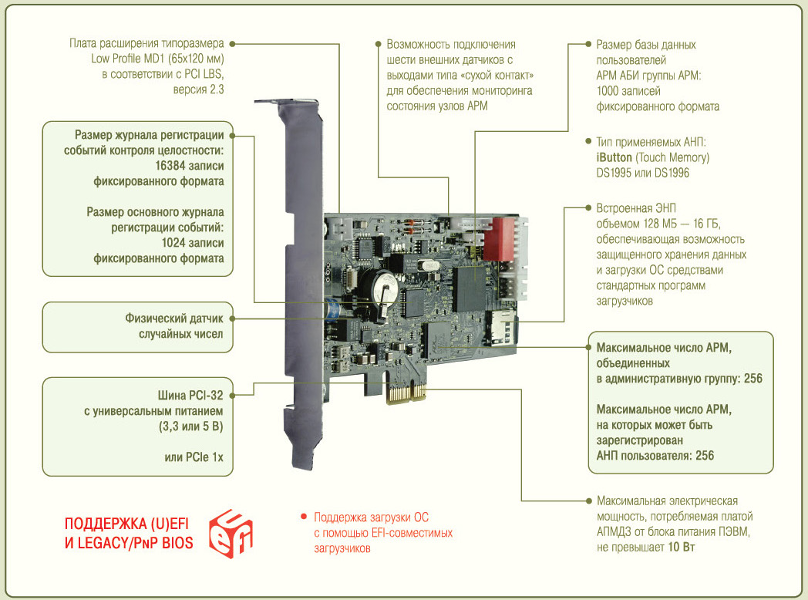
\includegraphics[width=\textwidth,height=\textheight,keepaspectratio]{images/apmdz.png}
    \caption{Пример специализированного аппаратного обеспечения: АПМДЗ Максим-М1 \cite{maksim} \label{fig:apmdz}}
\end{figure}


\begin{figure}[!htbp]
    \centering
    \begin{tikzpicture}[%
            start chain=going below,    % General flow is top-to-bottom
            node distance=6mm and 30mm, % Global setup of box spacing
            line/.style={draw, -latex'},
            every join/.style={line},
            block/.style={draw,
            on chain,
            on grid,
            rectangle,
            minimum height = 2em}
            ]
            \node [block, minimum width = 15cm] (feasibility)
            {Технико-экономическое обоснование};
            \node [block, minimum width = 15cm] (preliminary design) [below=2cm of feasibility]
            {Предварительныое проектирование};
            \node [block, minimum width = 15cm] (prototyping) [below=2cm of preliminary design]
            {Прототипирование};
            \node [block, minimum width = 15cm] (design for manufacturing) [below=2cm of prototyping]
            {Проектирование для производства и сборки};
            \node [block, minimum width = 15cm] (manufacturing) [below=2cm of design for manufacturing]
            {Производство};

            \draw [line] (feasibility) -- (preliminary design);
            \draw [line] (preliminary design) -- (prototyping);
            \draw [line] (prototyping) -- (design for manufacturing);
            \draw [line] (design for manufacturing) -- (manufacturing);

    \end{tikzpicture}
    \caption{Этапы создания аппаратного обеспечения}\label{fig:hardware-design}
\end{figure}

Создание аппаратного обеспечения -- трудоемкий процесс (\cref{fig:hardware-design}),
непременно сязанный с созданием прикладного программного обеспечения.
В свою очередь, отсутствие возможности исполнения ПО с использованием АО серьезно усложняет отладку и тестирование конечного продукта.

Прикладная польза от эмуляции аппаратного обеспечения может быть достигнута не только
при проектировании и разработке специализированного аппаратного обеспечения, но и, напрмер,
для совместного использования одного физического устройства несколькими компьютерами (в основном
виртуальными машинами).
Представляя аппаратное обеспечение гостевой системе как физическое устройство, можно
свести на нет затраты на написание специализированных драйверов и утилизировать
существующие, вынося обработку совместного использования в реализацию эмулируемого аппаратного обеспечения.

В частности, можно запустить некоторое количество виртуальных машин на одной физической, и для каждой
виртуальной машины использование графического ускорителя будет прозрачным, тогда как на самом
деле управлением задачами отрисовки или обработки данных будет заниматься виртуальное устройство.

Также вынесение интерфейса реального устройства в виртуальное позволяет создать систему с архитектурой,
где виртуальное устройство общается с программой-посредником,
которая уже отдает команды реальному устройству или группе устройств.
Например, запускать в виртуальной машине вычисления на виртуальных графических ускорителях, которые
будут, в свою очередь, отдавать задачи обсчета реальным графическим ускорителям где-нибудь в облаке.

Помимо перечисленных выше применений, виртуальные устройства предоставляются некоторыми компаниями
в режиме PaaS -- Platform as Service или <<Платформа как услуга>>, что позволяет другим разработчикам
испльзовать их для удаленного тестирования своих приложений в разных окружениях \cite{lambdatest,genymotion}.


\section{Эмуляция аппаратного обеспечения}\label{sec:ch1/sec1}

Тезис Чёрча-Тьюринга гласит: любая вычислимая (то есть та,
которая может быть реализована на машине Тьюринга) функция вычислима машиной Тьюринга.
Физический тезис Чёрча-Тьюринга гласит: любая функция, которая может быть вычислена физическим устройством, может быть вычислена машиной Тьюринга.

Существуют различное отношение к тезису Чёрча-Тьюринга.
Некоторые считают, что он может быть доказан, другие говорят, что он служит определением вычислений.
Несмотря на то, что тезис до сих пор не доказан, его верность исходит из того, что любая, открытая на текущий момент
реалистичная модель вычислений доказывала его правоту.

Тезис неразрывно связан с термином <<эмуляция>>.

Эмуляция -- это процесс имитирования поведения одного оборудования и/или программного обеспечения
на другом оборудовании и/или программном обеспечении.

Эмулятор АО может использоваться как для имитирования совершенно другого оборудования, так и того, на котором она проводится.
Например, большое количество принтеров умеет эмулировать линейку LaserJet компании Hewlett-Packard,
так как большая часть ПО разработана как раз под LaserJet.

Эмуляторы аппаратного обеспечения бывают разного назначения:

\paragraph{Симуляторы логики}\label{logic-sim}

Данный вид эмуляторов (пример на \cref{fig:metal-nes})
используется для исследования и верификации аппаратного обеспечения на различных уровнях:
\begin{itemize}
    \item компонентном;
    \item логических вентилей;
    \item регистровых передач;
\end{itemize}


\begin{figure}[!htbp]
    \centering
    \begin{adjustbox}{max totalsize={0.8\textwidth}{\textheight}}
        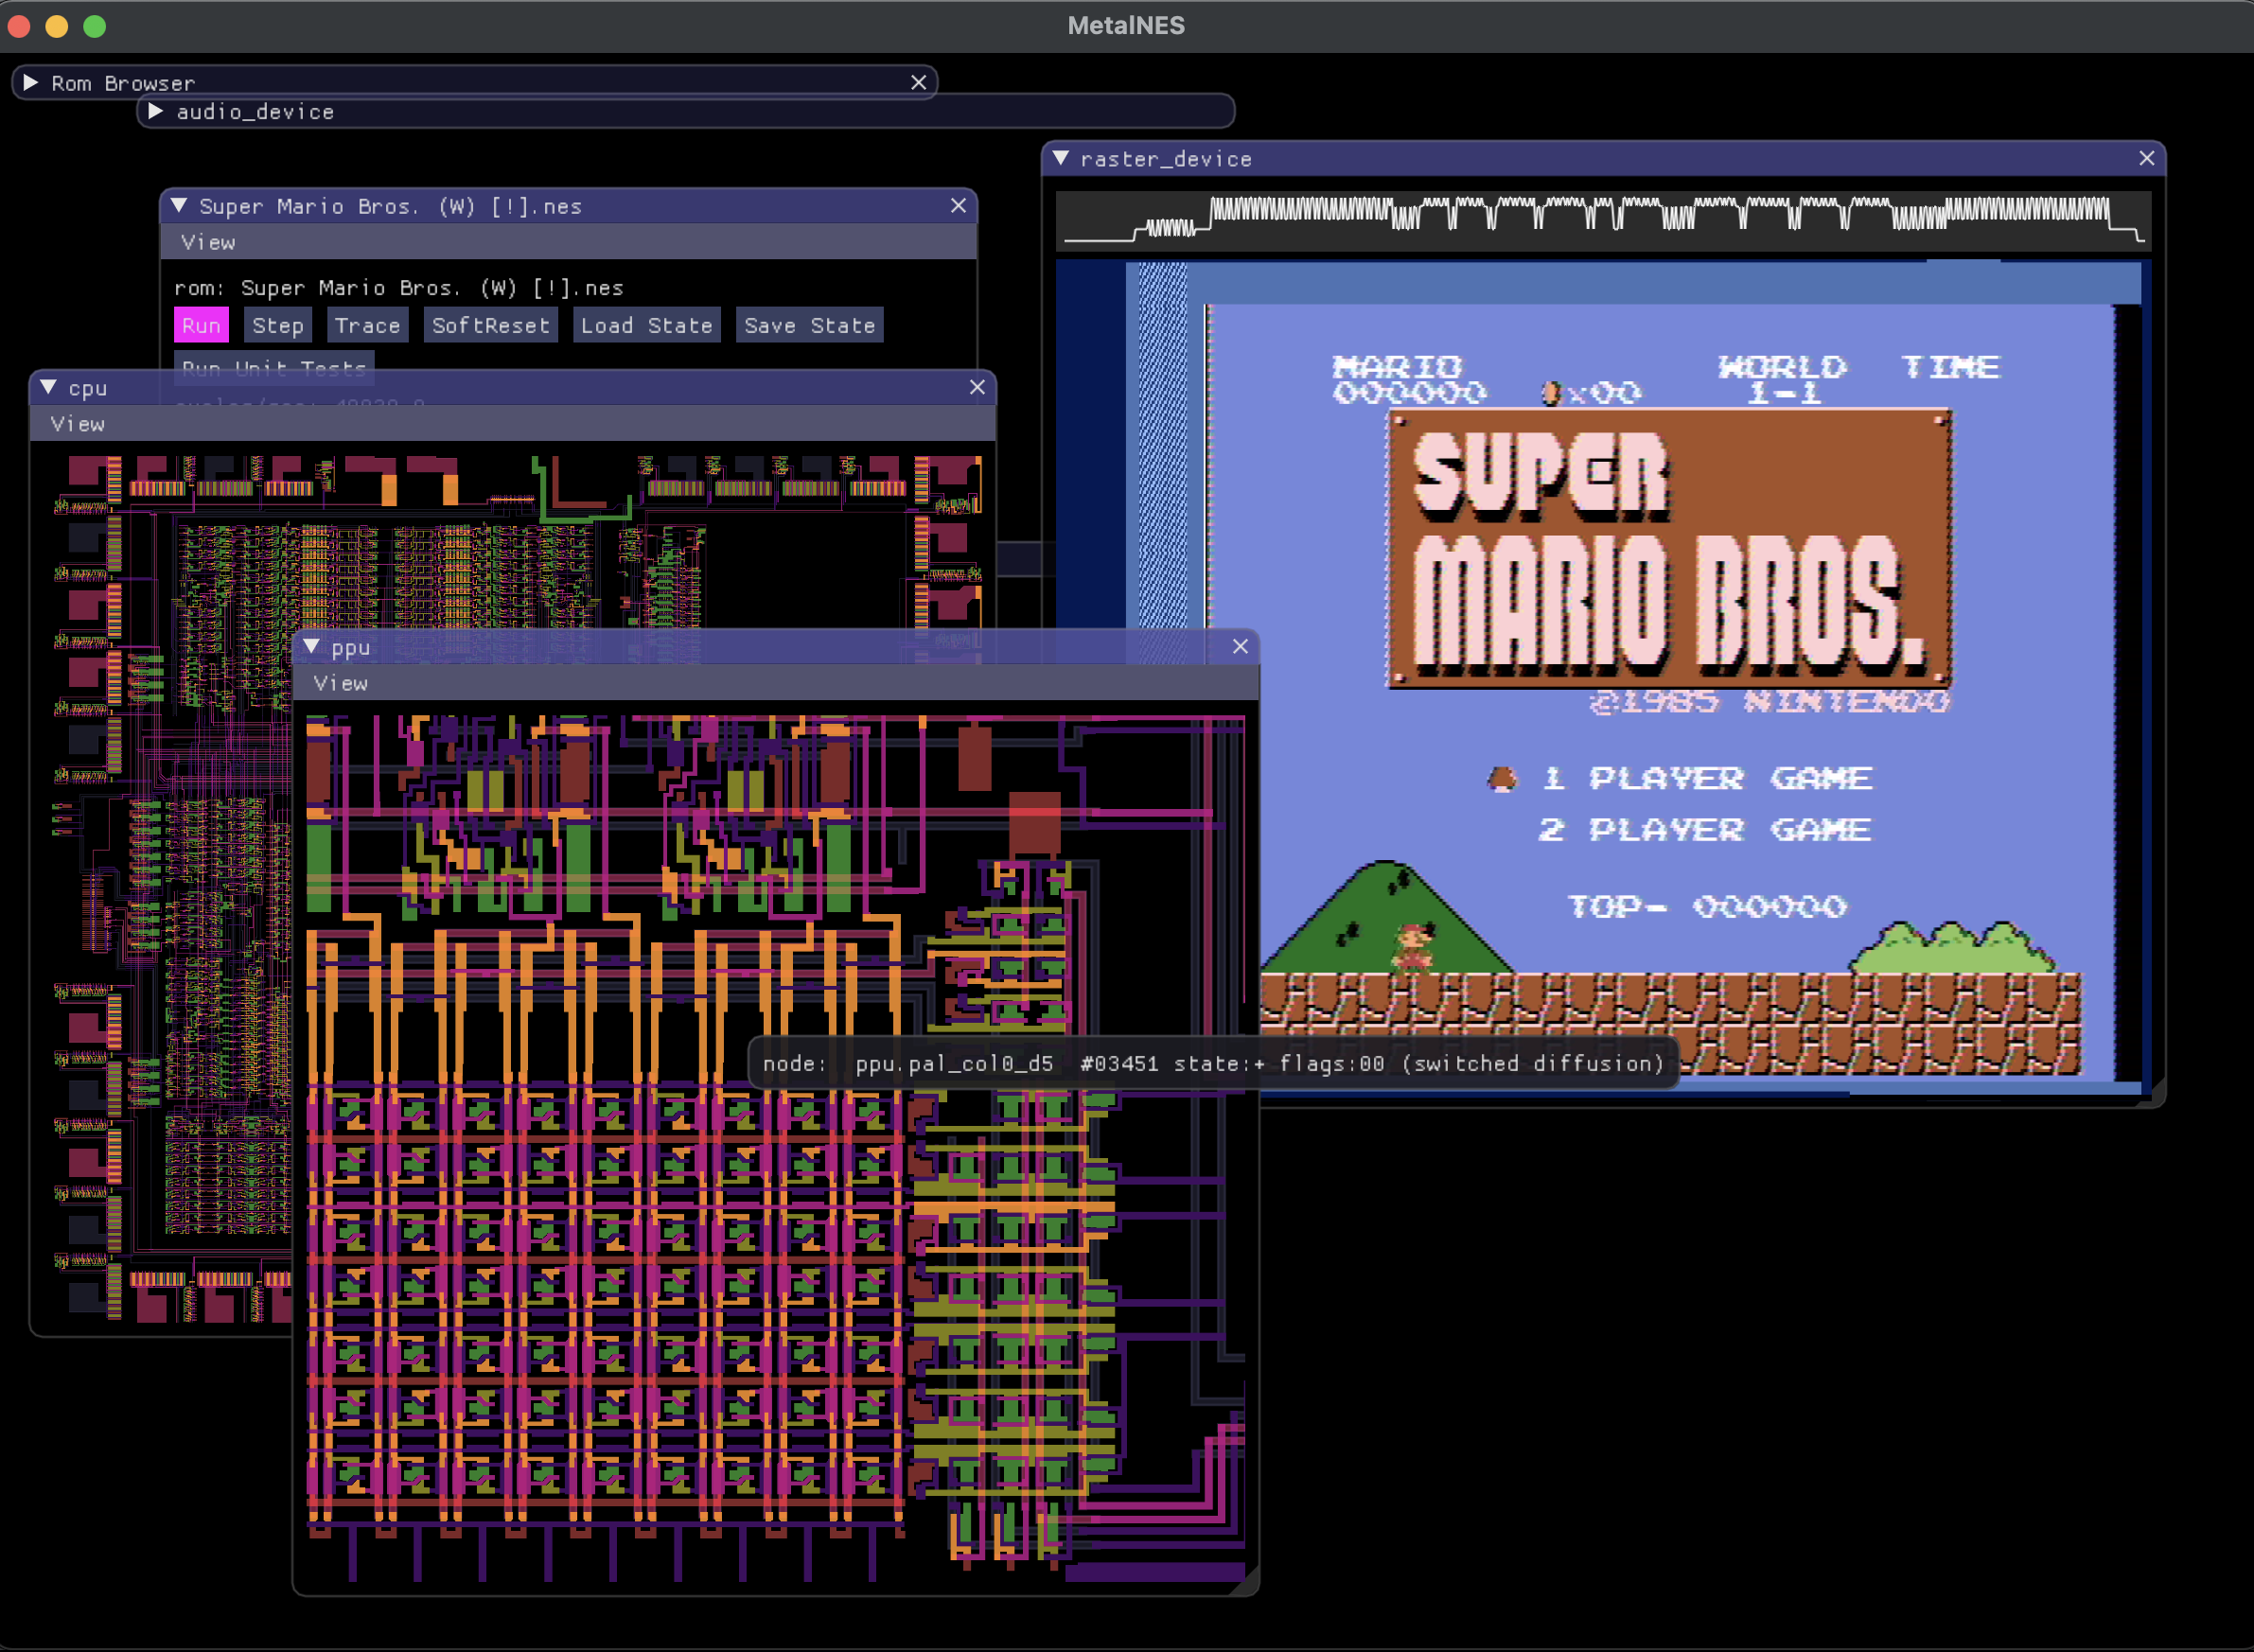
\includegraphics[]{images/metal-nes.png}
    \end{adjustbox}
    \caption{Симулятор игровой приставки NES транзисторного уровня \cite{metalnes}.}\label{fig:metal-nes}
\end{figure}

\paragraph{Высокоуровневые эмуляторы}\label{high-level-emu}

Высокоуровневая эмуляция -- это набор методов эмулирования некоторых компонентов целой системы.
Позволяет не исполнять инструкции или производить обработку данных один в один, как на целевом оборудовании,
заменяя <<горячие>> пути обработки аналогичными по результату.

Одними из первых данный подход был использован в эмуляторах игровых консолей, где команды отрисовки трёхмерной сцены
эмулировались не на процессоре, как все остальное оборудование консоли, а отдавались напрямую
графическому процессору машины, на которой происходил процесс эмуляции.


\paragraph{Эмуляторы процессора}\label{cpu-emu}

Эмулируют конкретную архитектуру процессора, позволяя запускать программы, не предназначенные для физического компьютера.
Зачастую умеют эмулировать не только процессор, но и переферийные устройства.


\paragraph{Эмуляторы терминала}\label{term-emu}

Эмулируют терминал компьютера внутри некоторой архитектуры отображения данных на дисплее.


\paragraph{Сэмуляторы}\label{sim-emu}

Являются симбиозом симуляторов и эмуляторов, который берет лучшее от двух миров.
Аппаратное обеспечение описовается HDL-языками, после чего данное описание оборудования симулируется на стендах.
Первоначальная функциональная верификация производится через симуляцию на уровне регистровых передач или логических вентилей.
В событийно-ориентированной симуляции инструкции последовательно исполняются процессором, потому что в превалирующем большинстве
сценариев не возможно провести данную симуляцию параллельно. Последовательный подход приводит к долгим симуляциям, особенно в
сложных системах на кристалле.
После симуляции описание регистровых передач должно быть зашито в аппаратное обеспечение (FPGA, ASIC).
Но идеализированное представление аппаратного обеспечения в симуляции отличается от реального аппаратного обеспечения.
Отличие между симуляцией и работой аппаратного обеспечения является серьезной причиной применений эмуляции при
проектировании.
Преимуществом данного метода является:
\begin{itemize}
    \item ускорение симуляции: часть сложной системы, не релевантная для симуляции переносится в эмулятор,
        что позволяет вынести из симуляции нерелевантные части;
    \item использование реального аппаратного обеспечения на ранних этапах проектирования;
\end{itemize}

Для создания виртуального аппаратного обеспечения могут использоваться различные подходы к эмуляции в зависимости
от цели эмулирования реального устройства.
В данной работе используется эмулятор процессора (\cref{cpu-emu}) -- QEMU \cite{qemu} из-за его открытости,
постоянной поддержки сообществом открытого ПО и имеющегося интерфейса встраивания
сторонних виртуальных устройств.


\subsection{Создание эмуляторов}\label{sec:ch1/sec1/sub2}

Создание эмуляторов -- трудоемкий и затратный процесс. Помимо перечисленных ранее типов эмуляторов особой популярностью
пользуются также эмуляторы игровых приставок, как старых, так и новых.
Их создание помогает сохранить игры и программы для будущих поколений, формируя целые виртуальные библиотеки, как,
например раздел в Internet Archive\cite{console-archive}, посвященный игровым приставкам.
С ростом вычислительной мощности усложняется и архитектура современных игровых приставок.
Эмулятор для PlayStation 4 вышел только через восемь лет после выхода самой консоли \cite{ps4-emulator}, и то
он не может запустить всю коллекцию игр, а PlayStation 4 не принадлежит последнему поколению приставок.

Создание эмуляторов какого-либо аппаратного обеспечения укладывается в следующих этапах,
показанных на \cref{fig:emu-creation-naive}.

\begin{figure}[!htbp]
    \centering
    \begin{tikzpicture}[%
            start chain=going below,    % General flow is top-to-bottom
            node distance=6mm and 30mm, % Global setup of box spacing
            line/.style={draw, -latex'},
            every join/.style={line},
            block/.style={draw,
            on chain,
            on grid,
            rectangle,
            minimum height = 2em}
            ]
            \node [block, minimum width = 16cm] (subset)
            {Вычленение эмулируемого подмножества функционала устройства};
            \node [block, minimum width = 16cm, fill=yellow] (conversation) [below=2cm of subset]
            {Выбор и написание средства общения ПО с эмулятором};
            \node [block, minimum width = 16cm] (logic) [below=2cm of conversation]
            {Написание логики эмулятора};

            \draw [line] (subset) -- (conversation);
            \draw [line] (conversation) -- (logic);

    \end{tikzpicture}
    \caption{Этапы создания эмулятора аппаратного обеспечения}\label{fig:emu-creation-naive}
\end{figure}

%\begin{enumerate}[label={\arabic*)}]
%    \item вычленения эмулируемого подмножества функционала устройства;
%    \item выбора и написания средства общения ПО с эмулятором;
%    \item .
%\end{enumerate}

Первый этап является проектировочным и его результат зависит от нужд конкретной реализации, временных ограничений,
соображений о целесообразности.
Второй этап тоже, до некоторой степени, проектировочный, но уже здесь можно принять решение
воспользоваться эмуляторами, которые поддерживают встраивание виртуального аппаратного обеспечения,
что автоматически решит задачу.
Третий этап является полностью практическим.

Облегчить второй и третий этап можно, если решить использовать уже имеющуюся инфраструктуру эмулятора,
встроив в нее эмулируемое аппаратное обеспечение.
Использование имеющейся инфраструктуры задает строгий интерфейс встраивания, что ограничивает и тривиализирует
общение ПО с виртуальным устройством.
Помимо этого, интерфейс встраивания позволяет автоматически генерировать если не всю, то часть взаимодействия
между виртуальным устройством и эмулятором.

Используя данный подход, задача создания эмулятора аппаратного обеспечения трансформируется в следующие этапы,
\cref{fig:emu-creation-pro}.

\begin{figure}[!htbp]
    \centering
    \begin{tikzpicture}[%
            start chain=going below,    % General flow is top-to-bottom
            node distance=6mm and 30mm, % Global setup of box spacing
            line/.style={draw, -latex'},
            every join/.style={line},
            block/.style={draw,
            on chain,
            on grid,
            rectangle,
            minimum height = 2em}
            ]
            \node [block, minimum width = 17cm] (subset)
            {Вычленение эмулируемого подмножества функционала устройства};
            \node [block, minimum width = 17cm, fill=yellow] (conversation) [below=2cm of subset]
            {Реализация общения виртуального аппаратного обеспечения и эмулятора};
            \node [block, minimum width = 17cm, fill=yellow] (driver) [below=2cm of conversation]
            {Реализация общения ПО с эмулятором (написание драйвера)};
            \node [block, minimum width = 17cm] (logic) [below=2cm of driver]
            {Написание логики эмулятора};

            \draw [line] (subset) -- (conversation);
            \draw [line] (conversation) -- (driver);
            \draw [line] (driver) -- (logic);

    \end{tikzpicture}
    \caption{Этапы создания эмулятора аппаратного обеспечения с использованием существующего эмулятора}\label{fig:emu-creation-pro}
\end{figure}

%\begin{enumerate}[label={\arabic*)}]
%    \item вычленения эмулируемого подмножества функционала устройства;
%    \item реализация общения виртуального аппаратного обеспечения и эмулятора;
%    \item реализация общения ПО с эмулятором (написание драйвера);
%    \item написание логики эмулятора.
%\end{enumerate}

Несмотря на увеличение количества этапов, второй и третий этап данной схемы реализовать проще и
целесообразнее, чем второй этап предыдущей схемы, так как во первом случае
протокол общения прикладного ПО и аппаратного обеспечения будет находиться частично в
эмуляторе аппаратного обеспечения, частично в прикладном ПО.
Тогда как во втором случае протокол это реализации драйвера устройства, который в любом случае придется писать.

Но даже в таком подходе можно облегчить второй и четвертый этапы, для этого не хватает только
генератора, который мог бы самостоятельно встроить будущее виртуальное аппаратное обеспечение
в эмулятор, основываясь на спецификации устройства.
Существование такого генератора не только полностью бы убрало второй этап, но и облегчило последний.
В случае, если есть возможность получить описание работы эмулируемого аппаратного обеспечения на HDL-языке,
то четвертый этап создания эмулятора тоже автоматизируется, так как логика работы аппаратного обеспечения
уже описана на HDL-языке.


\section{Точки зрения других авторов}\label{sec:ch1/sec2}

В работе <<Автоматизация разработки моделей устройств и вычислительных машин для QEMU>> \cite{imposters}
авторы рассматривают устройство и способы автоматизации рутинных этапов добавления виртуального
аппаратного обеспечения в известный эмулятор с открытым исходным кодом -- QEMU.
Авторами обозначена потребность коллективов разработчиков в универсальном средстве
для создания виртуального аппаратного обеспечения,
разработаны графические и консольные утилиты по генерации виртуальных устройств
в соответствии с объектной моделью QEMU.

В отличие от данной работы, авторы выделяют проблему анализа и отладки машинного кода,
в том числе и специфического, компьютерных вирусов, в котором эмулятор <<даёт дополнительный
<<рубеж>> изоляции между исследуемым кодом и инструментами анализа>>.

Задумка исследования \cite{imposters} состоит в создании виртуального аналога некоторого реального стенда
с определенным набором специальных аппаратных средств со следующим процессом:

<<С использованием разработанного инструмента процесс разработки как модели устройства,
так и VM принимает следующую форму.
Его можно разбить на 4 этапа: \textit{ознакомление} с документацией, \textit{подготовка} эмулятора,
\textit{генерация} заготовок интерфейсной части и \textit{реализация} индивидуальной части.
При ознакомлении с документацией задача разработчика: оценить состав
машины: какие устройства потребуется реализовать, как их связать в единую
VM и т. д. Эта информация потребуется для генерации заготовок. Поскольку
инструмент генерирует заготовки с учётом текущей версии кода QEMU,
может потребоваться внесение подготовительных изменений в код, чтобы
задействовать максимум возможностей инструмента. Например, добавление
новых идентификаторов PCI. Затем, разработчик задаёт параметры и получает
заготовки — выполняет этап генерации. Наконец, он переходит к реализации
индивидуальных частей кода устройств и уточнению заготовок VM. При этом
происходит более детальное изучение документации, отладка и
корректирование кода.>>

Корректирование C-кода ведет к серьезным потенциальным ошибкам (\cref{fig:curl-c-issues}) в реализации \cite{qemu-c-style}.
Чтобы уменьшить вероятность ошибок программирования, стоит применить некий встраиваемый
высокоуровневый язык программирования, вроде Python \cite{python} или Lua \cite{lua},
который позволит оперировать конструкциями и коллекциями, проверяющими условия доступа.
Потенциально это так же сохранит компактность кодовой базы,
правда, за счет некоторого уменьшения производительности. \label{better-logic}
Язык Nim \cite{nim} сочетает в себе парадигмы Python с компиляцией исходного кода в машинный через
промежуточную компиляцию в C. К сожалению, язык, несмотря на быстроту и удобство, обладает
недостатками: большие файлы автогенерированного C-кода, которые требуется включать в сборку QEMU,
неустоявшаяся стандартная библиотека и малое количество сторонних модулей.

\begin{figure}[!htbp]
    \centering
    \begin{adjustbox}{max totalsize={0.8\textwidth}{\textheight}}
        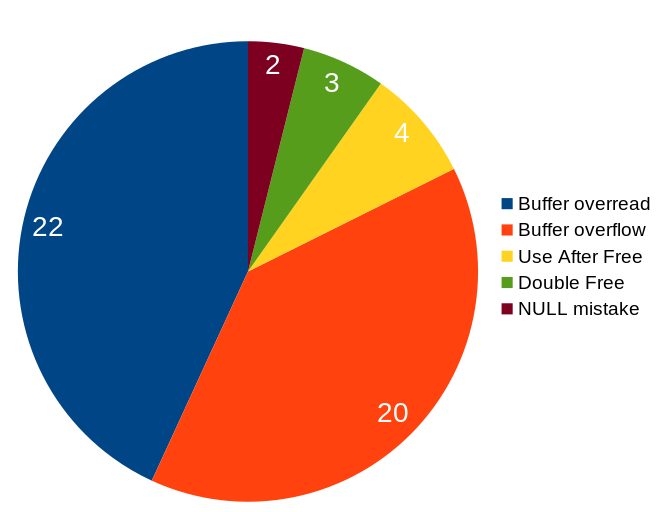
\includegraphics[]{images/curl-c-issues.png}
    \end{adjustbox}
    \caption{Половина уязвимостей популярной библиотеки curl \cite{curl}
    являются классическими ошибками C \cite{curl-errors}.}\label{fig:curl-c-issues}
\end{figure}

ИСП РАН имеет несколько программных решений на основе QEMU, позволяющих не только отлаживать и исследовать
машинный код внутри эмулятора, но и ускоряющих разработку новых архитектур \cite{imposters-toolset}.
Автору данной научной работы кажется, что дальнейшим улучшением пользовательского опыта в части анализа машинного кода
и реверсивной отладки будет заимствование некоторых идей у <<вневременного отладчика>> qira \cite{qira}.
Qira позиционируется как инструмент для вневременной отладки (Timeless Debugging) и имеет Web-интерфейс.
Qira тоже основан QEMU и работает через эмуляцию пользовательского пространства (User-space emulation).
Эмуляция пользовательского пространства позволяет запускать в целевой системе программы,
предназначенные для других архитектур, не прибегая к эмуляции ОС.
Это достигается за счет эмуляции только процессора, на которую рассчитана запускаемая
программа, все системные вызовы программы перенаправляются ядру целевой ОС.

\begin{figure}[!htbp]
    \centering
    \begin{adjustbox}{max totalsize={0.8\textwidth}{\textheight}}
        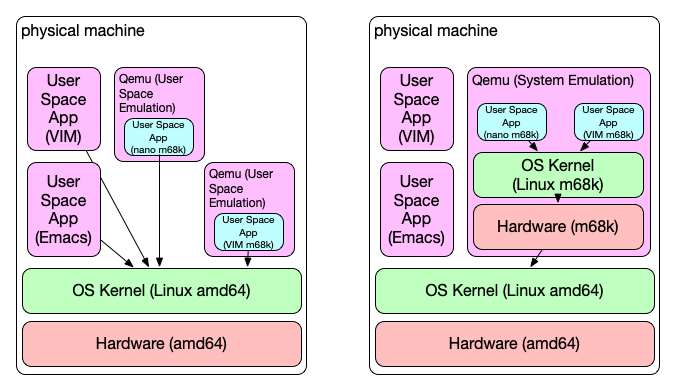
\includegraphics[]{images/qemu-userspace.png}
    \end{adjustbox}
    \caption{Сравнение эмуляции полноценной системы и пользовательского пространства для отдельной программы}\label{fig:qemu-userspace}
\end{figure}

Инструмент ИСП РАН основан на версии QEMU 2019 года, и зафиксирован на определенном коммите в системе
контроля версий git. С того момента прошло уже довольно много времени: было изменено 7975 файлов, с 1659755 изменениями в целом.
За это время поменялась и система сборки -- QEMU перешел с Makefile'ов на Meson, поэтому
использовать автоматическое встраивание инструмента в систему сборки не получится.

\subsection{Вневременная отладка}\label{sec:ch1/sec2/sub1}

<<Вневременная>> или Timeless (Time-travel) отладка подразумевает предварительную запись работы программы и
последующее отлаживание уже сделанной записи. Это позволяет точно детектировать ошибки, отлавливать и
анализировать недетерминированные ситуации, вроде ошибок, связанных с многопоточностью, работой с
устройствами ввода-вывода или сетью. Также вневременная отладка позволяет <<ходить>> по исполнению
программы не только вперед, но и назад, то есть исполнять команды в реверсивном порядке.

На данный момент QEMU поддерживает эмуляцию пользовательского пространства только в Linux и BSD.
Разница между эмуляцией пользовательского пространства и полноценной системы показана на 
\cref{fig:qemu-userspace}.
Плюсами такого решения являются:
\begin{itemize}
    \item прозрачная интеграция программ в целевую систему;
    \item лучшее, по сравнению с эмуляцией всей системы, использование процессора и памяти;
    \item улучшенная производительность, так как не нужно эмулировать аппаратное обеспечение и ОС.
\end{itemize}


\section{Обоснование плана диссертационных исследований}\label{sec:ch1/sec3}

План диссертационных исследований состоит в:

\begin{enumerate}[label={\arabic*)}]
    \item исследовании существующих решений по созданию виртуального аппаратного обеспечения;
    \item выборе программного решения, которое наиболее полно покроет требования к функционалу;
    \item декомпозиции поставленной задачи для создания методики и алгоритма генерации виртуального аппаратного обеспечения;
    \item создании методики и алгоритма генерации виртуального аппаратного обеспечения на основе его спецификации;
    \item разработке лингвистического аппарата (семантика, синтаксис) языка для создания программ по генерации виртуального
        аппаратного обеспечения;
    \item анализе эффективности методики и алгоритма.
\end{enumerate}

В качестве альтернативных решений рассматривался подход <<записи и воспроизведения>> (используется в umockdev \cite{umockdev}),
Плюсом данного подхода является отсутствие необходимости программировать и описывать виртуальное устройство,
но большие недостатки: необходимость физического наличия устройства для первоначальной записи
поведения, детерминированность и ограниченность Linux-системами выводят данный вариант из рассмотрения.

\subsection{Использование эмулятора с открытым исходным кодом}\label{sec:ch1/sec4/sub1}

Использование эмулятора с открытым исходным кодом является обязятельным
условием для встраивания собственного виртуального аппаратного обеспечения.
Активно развивающихся эмуляторов с открытым исходным кодом мало, Bochs \cite{bochs} и QEMU
единственные, которые можно было бы использовать для создания на их основе
эмуляторов аппаратного обеспечения.

Несмотря на то, что Bochs, как и QEMU, является кроссплатформенным эмулятором,
для решения создания виртуального аппаратного обеспечения
он не подходит в виду поддержки только архитектуры x86, низкой скорости эмуляции
и отсутствия удобного интерфейса для встраивания собственных устройств.
Исходя из этого, лучшим эмулятором для поставленной задачи будет QEMU.

\section{Унифицированный подход к созданию виртуального аппаратного обеспечения в QEMU}\label{sec:ch1/sec4}

Унифицированный подход к созданию виртуального аппаратного обеспечения в QEMU позволяет
повысить степень автоматизации и корректности рутинной работы по внедрению
эмулятора в исполняемую среду.

Помимо этого требуется понизить не только порог вхождения для встраивания виртуального аппаратного обеспечения
в выбранный эмулятор, но время имплементации логики устройства и вероятность ошибкок программирования\cref{better-logic}.
Значительная часть всех уязвимостей эмулятора QEMU связана не с проблемами архитектуры или эмуляции,
а с классическами ошибками, которые совершают Си-программисты в реализации устройств.


Для понижения порога вхождения, уменьшения возможных ошибок программирования,
связанных с управлением памятью, автоматизации создания интерфейса виртуального
устройства, предполагается создать проблемно-ориентированный язык (DSL), который позволит
описывать виртуальные как интерфейс виртуальных устройств, так и их логику.

Центральным элементом данной системы будет использован скриптовый язык Python, прозрачно интегрируемый
в итоговое устройство для исполнения логики работы устройства.
Данный язык выбран из-за хорошей интеграции с языком C, всеобщей распространенности и большого
количества сторонних библиотек, поддерживающихся большим сообществом разработчиков.
Как раз использование сторонних библиотек высокого уровня позволит создавать устройства
высокой гибкости и повысит скорость разработки.


%\subsection{Симуляция HDL}\label{sec:ch1/sec4/sub1}
%
%HDL или Harwdare Description Language -- специализированный язык для описания структуры и поведния
%электронных схем. Самыми известными и популярными представителями являются Verilog и VHDL.
%Данный тип языков помогает разрабатывать электронные схемы на более высоком уровне абстракции, чем раньше,
%что просто необходимо при проектировании сложных современных интегральных схем.
%
%Процесс превращения HDL-кода в соединения логических вентилей называется логическим синтезом.
%Результат логического синтеза -- список соединений, который может быть зашит на ПЛИС, или исполнен в симуляторе, что позволяет
%протестировать HDL-программу не используя ПЛИС.
%
%\begin{figure}[!htbp]
%    \centering
%    \begin{adjustbox}{max totalsize={0.6\textwidth}{0.6\textheight}}
%        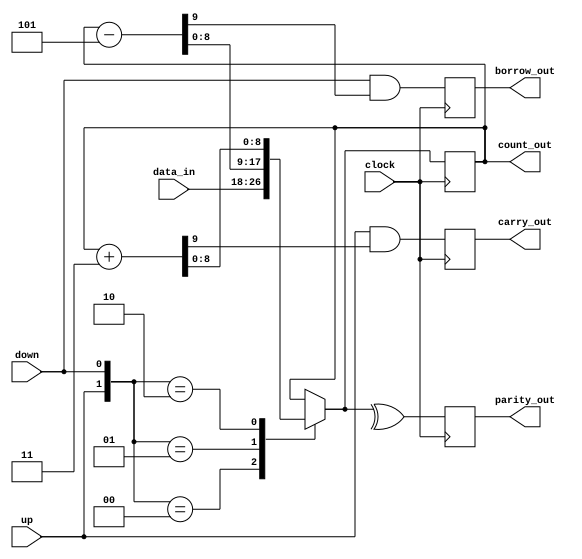
\includegraphics[]{images/netlist.png}
%    \end{adjustbox}
%    \caption{Визуализация результата логического синтеза}\label{fig:emu-creation-pro}
%\end{figure}
%
%
%Так как в списке соединений заложена логика работы устройства, пусть и на элементном уровне,
%то его можно использовать для эмуляции работы устройства.
%
%

%\subsection{Процесс добавления целевого аппаратного обеспечения в QEMU}\label{sec:ch1/sec4/sub2}

% Написать про устройство QEMU
% Написать про QOM
% Написать про Встраивание в QOM

\subsection{Архитектура QEMU}\label{sec:ch1/sec4/sub2/sub1}

QEMU (Quick Emulator) -- эмулятор аппаратного обеспечения различных платформ.
QEMU по-умолчанию использует TCG \cite{tcg} (\cref{fig:qemu-tcg}) или Tiny Code Generator (Маленький Генератор Кода) для
перевода инструкций эмулируемой системы в инструкции физической машины.

В процессе своей работы TCG разбивает поток инструкций на блоки, разделенные инструкциями
ветвления или вызова процедур.
В свою очередь, скомпилированные блоки переносятся в кэш трансляции и переиспользуются при следующих
вызовах, что ускоряет работу эмулятора.
TCG работает только с 32 и 64 битными операндами.

\begin{figure}[!htbp]
    \centering
    % !TEX encoding = UTF-8 Unicode
% Úτƒ-8 encoded
% http://www.linux.org.ru/forum/general/10357036
\tikzset{
    line/.style={draw, -latex'},
    every join/.style={line},
    u/.style={anchor=south},
    r/.style={anchor=west},
    fxd/.style={text width = 6em},
    it/.style={font={\small\itshape}},
    bf/.style={font={\small\bfseries}},
}
\tikzstyle{base_long} =
    [
        draw,
        on chain,
        on grid,
        align=center,
        minimum height=4ex,
        minimum width = 10ex,
        node distance = 6mm and 60mm,
        text badly centered,
    ]
\tikzstyle{base} =
    [
        draw,
        on chain,
        on grid,
        align=center,
        minimum height=4ex,
        minimum width = 10ex,
        text badly centered,
    ]
\tikzstyle{coord} =
    [
        coordinate,
        on chain,
        on grid
    ]
\tikzstyle{cloud} =
    [
        base,
        ellipse,
        node distance = 3cm,
        minimum height = 2em,
        text width=2cm
    ]
\tikzstyle{decision} =
    [
        base,
        diamond,
        aspect=2,
        node distance = 2cm,
        inner sep = 0pt
    ]
\tikzstyle{block} =
    [
        rectangle,
        base,
        rounded corners,
        minimum height = 2em
    ]
\tikzstyle{print_block} =
    [
        base,
        tape,
        tape bend top=none,
    ]
\tikzstyle{io} =
    [
        base,
        trapezium,
        trapezium left angle = 70,
        trapezium right angle = 110,
    ]
\tikzstyle{prompt} =
    [
        base,
        trapezium,
        trapezium left angle = 90,
        trapezium right angle = 80,
        shape border rotate = 90
    ]
\tikzstyle{disk file} =
    [
        base,
        cylinder,
        aspect=0.2,
    ]
\tikzstyle{process} =
    [
        rectangle,
        base,
    ]
\makeatletter
\pgfkeys{/pgf/.cd,
    subrtshape w/.initial=2mm,
    cycleshape w/.initial=2mm
}
\pgfdeclareshape{parallelshape}{
    \inheritsavedanchors[from=rectangle]
    \inheritanchorborder[from=rectangle]
    \inheritanchor[from=rectangle]{north}
    \inheritanchor[from=rectangle]{center}
    \inheritanchor[from=rectangle]{west}
    \inheritanchor[from=rectangle]{east}
    \inheritanchor[from=rectangle]{mid}
    \inheritanchor[from=rectangle]{base}
    \inheritanchor[from=rectangle]{south}
    \backgroundpath{
        \southwest \pgf@xa=\pgf@x \pgf@ya=\pgf@y
        \northeast \pgf@xb=\pgf@x \pgf@yb=\pgf@y
        \def\ppd@offset{\pgfpoint{\pgfutil@tempdima}{0ex}}
        \def\ppd@offsetm{\pgfpoint{-\pgfutil@tempdima}{0ex}}
        \pgfpathmoveto{\pgfqpoint{\pgf@xa}{\pgf@ya}}
            \pgfpathlineto{\pgfqpoint{\pgf@xb}{\pgf@ya}}
        \pgfpathclose
        \pgfpathmoveto{\pgfqpoint{\pgf@xb}{\pgf@yb}}
            \pgfpathlineto{\pgfqpoint{\pgf@xa}{\pgf@yb}}
        \pgfpathclose
    }
}
\pgfdeclareshape{subrtshape}{
    \inheritsavedanchors[from=rectangle]
    \inheritanchorborder[from=rectangle]
    \inheritanchor[from=rectangle]{north}
    \inheritanchor[from=rectangle]{center}
    \inheritanchor[from=rectangle]{west}
    \inheritanchor[from=rectangle]{east}
    \inheritanchor[from=rectangle]{mid}
    \inheritanchor[from=rectangle]{base}
    \inheritanchor[from=rectangle]{south}
    \backgroundpath{
        \southwest \pgf@xa=\pgf@x \pgf@ya=\pgf@y
        \northeast \pgf@xb=\pgf@x \pgf@yb=\pgf@y
        \pgfmathsetlength\pgfutil@tempdima{\pgfkeysvalueof{/pgf/subrtshape w}}
        \def\ppd@offset{\pgfpoint{\pgfutil@tempdima}{0ex}}
        \def\ppd@offsetm{\pgfpoint{-\pgfutil@tempdima}{0ex}}
        \pgfpathmoveto{\pgfqpoint{\pgf@xa}{\pgf@ya}}
        \pgfpathlineto{\pgfqpoint{\pgf@xb}{\pgf@ya}}
        \pgfpathlineto{\pgfqpoint{\pgf@xb}{\pgf@yb}}
        \pgfpathlineto{\pgfqpoint{\pgf@xa}{\pgf@yb}}
        \pgfpathclose
        \pgfpathmoveto{\pgfpointadd{\pgfpoint{\pgf@xa}{\pgf@yb}}{\ppd@offsetm}}
        \pgfpathlineto{\pgfpointadd{\pgfpoint{\pgf@xa}{\pgf@ya}}{\ppd@offsetm}}
        \pgfpathlineto{\pgfpointadd{\pgfpoint{\pgf@xb}{\pgf@ya}}{\ppd@offset}}
        \pgfpathlineto{\pgfpointadd{\pgfpoint{\pgf@xb}{\pgf@yb}}{\ppd@offset}}
        \pgfpathclose
    }
}
\pgfdeclareshape{cyclebegshape}{
    \inheritsavedanchors[from=rectangle]
    \inheritanchorborder[from=rectangle]
    \inheritanchor[from=rectangle]{north}
    \inheritanchor[from=rectangle]{center}
    \inheritanchor[from=rectangle]{west}
    \inheritanchor[from=rectangle]{east}
    \inheritanchor[from=rectangle]{mid}
    \inheritanchor[from=rectangle]{base}
    \inheritanchor[from=rectangle]{south}
    \backgroundpath{
        \southwest \pgf@xa=\pgf@x \pgf@ya=\pgf@y
        \northeast \pgf@xb=\pgf@x \pgf@yb=\pgf@y
        \pgfmathsetlength\pgfutil@tempdima{\pgfkeysvalueof{/pgf/cycleshape w}}
        \pgfpathmoveto{\pgfqpoint{\pgf@xa}{\pgf@ya}}
\pgfpathlineto{\pgfpointadd{\pgfpoint{\pgf@xa}{\pgf@yb}}{\pgfpoint{0ex}{-\pgfutil@tempdima}}}
\pgfpathlineto{\pgfpointadd{\pgfpoint{\pgf@xa}{\pgf@yb}}{\pgfpoint{\pgfutil@tempdima}{0ex}}}
\pgfpathlineto{\pgfpointadd{\pgfpoint{\pgf@xb}{\pgf@yb}}{\pgfpoint{-\pgfutil@tempdima}{0ex}}}
\pgfpathlineto{\pgfpointadd{\pgfpoint{\pgf@xb}{\pgf@yb}}{\pgfpoint{0ex}{-\pgfutil@tempdima}}}
\pgfpathlineto{\pgfqpoint{\pgf@xb}{\pgf@ya}}
        \pgfpathclose
    }
}
\pgfdeclareshape{cycleendshape}{
    \inheritsavedanchors[from=rectangle]
    \inheritanchorborder[from=rectangle]
    \inheritanchor[from=rectangle]{north}
    \inheritanchor[from=rectangle]{center}
    \inheritanchor[from=rectangle]{west}
    \inheritanchor[from=rectangle]{east}
    \inheritanchor[from=rectangle]{mid}
    \inheritanchor[from=rectangle]{base}
    \inheritanchor[from=rectangle]{south}
    \backgroundpath{
        \southwest \pgf@xa=\pgf@x \pgf@ya=\pgf@y
        \northeast \pgf@xb=\pgf@x \pgf@yb=\pgf@y
        \pgfmathsetlength\pgfutil@tempdima{\pgfkeysvalueof{/pgf/cycleshape w}}
        \pgfpathmoveto{\pgfqpoint{\pgf@xb}{\pgf@yb}}
\pgfpathlineto{\pgfpointadd{\pgfpoint{\pgf@xb}{\pgf@ya}}{\pgfpoint{0ex}{\pgfutil@tempdima}}}
\pgfpathlineto{\pgfpointadd{\pgfpoint{\pgf@xb}{\pgf@ya}}{\pgfpoint{-\pgfutil@tempdima}{0ex}}}
\pgfpathlineto{\pgfpointadd{\pgfpoint{\pgf@xa}{\pgf@ya}}{\pgfpoint{\pgfutil@tempdima}{0ex}}}
\pgfpathlineto{\pgfpointadd{\pgfpoint{\pgf@xa}{\pgf@ya}}{\pgfpoint{0ex}{\pgfutil@tempdima}}}
\pgfpathlineto{\pgfqpoint{\pgf@xa}{\pgf@yb}}
        \pgfpathclose
    }
}
\makeatother
\tikzstyle{subroutine} =
    [
        base,
        subrtshape,
    ]
\tikzstyle{cyclebegin} =
    [
        base,
        cyclebegshape,
    ]
\tikzstyle{cycleend} =
    [
        base,
        cycleendshape,
    ]
\tikzstyle{connector} =
    [
        base,
        circle,
    ]

\tikzstyle{parallel} =
    [
        base_long,
        parallelshape,
    ]

\def\code (#1,#2) at (#3,#4) {
  \node [rectangle, base] (begin) at (#3,#4) {...};
  \node [rectangle, base] (left branch) [below left = 2cm of begin] {...};
  \node [rectangle, base] (right branch) [below right = 2cm of begin] {...};

  \coordinate (CENTER) at ($(left branch)!0.5!(right branch)$);

  \node [rectangle, base] (end) [below of = CENTER] {...};

  \draw [->] (begin) -- (left branch);
  \draw [->] (begin) -- (right branch);

  \draw [->] (left branch) -- (end);
  \draw [->] (right branch) -- (end);

  \node [draw, loosely dashed, thick, minimum width=6cm, minimum height=4cm] at (CENTER) {};
  \node [above=2cm of CENTER] {#2};
}

\begin{tikzpicture}[%
    start chain=going below,    % General flow is top-to-bottom
    node distance=6mm and 30mm, % Global setup of box spacing
    scale=0.7
    ]
    \code (emulated, Код эмулируемой системы) at (0,0)
    \code (native, Сгенерированный код) at (16,1.5)

    \draw [->] +(4.3,-2) -- (7,-2);
    \node [draw] (TCG) at (8,-2) {TCG};
    \draw [->] +(9,-2) -- (11.7,-2);

    \node [draw, loosely dashed, thick, minimum width=7cm, minimum height=5cm] (translation cache) at (16,-1.5) {};
    \node [above= 0.2cm of translation cache] {Кэш трансляции};

    \node [draw, minimum width=2cm, minimum height=2cm] at (0,-10) {QEMU};
    \node [draw] (prologue) at (7,-9) {пролог вызова};
    \node [draw] (epilogue) at (7,-11) {эпилог вызова};

    \coordinate (peCENTER) at ($(prologue)!0.5!(epilogue)$);

    \draw [->] (1.45,-9) -- (4.5,-9);
    \draw [->] (4.5,-11) -- (1.45,-11);

    \node [draw, loosely dashed, thick, minimum width=4cm, minimum height=3cm] (prologue epilogue) at (peCENTER) {};
    \node [above=0.2cm of prologue epilogue] {Передача контроля эмулятора};

    \draw [->] (prologue) -- (12,-9) -- (12, 0) -- (14.45, 0);
    \draw [->] (16, -4.35) -- (16, -11) -- (epilogue);


\end{tikzpicture}

    \caption{Схема работы QEMU TCG}\label{fig:qemu-tcg}
\end{figure}

Также TCG применяет оптимизацию к компилируемым блокам:
\begin{itemize}
    \item <<долгие>> инструкции заменяются на более быстрые альтернативы (если таковые имеются);
    \item производится анализ времени жизни переменных на уровне блока, при котором
        удаляются инструкции, не влияющие на вычисления.
\end{itemize}

Применение TCG позволяет запускать инструкции, предназначенные для любой поддерживаемой архитекуры
на любой другой поддерживаемой архитектуре, так как инструкции гостевой системы выполняются на виртуальных процессорах.
Это позволяет запускать любые операционные системы и приложения даже на старых процессорах, в которых нет поддержки
аппаратной виртуализации, хотя производительность виртуальной машины будет крайне низкая.
В случае, когда архитектура эмулируемой и физической системы совпадает, QEMU может применяться как средство виртуализации
и использовать аппаратное ускорение.
Здесь QEMU может использовать различные ускорители (гипервизоры, \cref{fig:kvm}),
отличающиеся в зависимости от операционной системы, в которой эмулятор запущен.
Гипервизор используется как <<прокладка>> для запуска некоторого программного обеспечения в виртуальной среде,
скрывая от данного программного обеспечения аппаратное обеспечение машины, на котором это ПО работает.

\begin{figure}[!htbp]
    \centering
    % !TEX encoding = UTF-8 Unicode
% Úτƒ-8 encoded
% http://www.linux.org.ru/forum/general/10357036
\tikzset{
    line/.style={draw, -latex'},
    every join/.style={line},
    u/.style={anchor=south},
    r/.style={anchor=west},
    fxd/.style={text width = 6em},
    it/.style={font={\small\itshape}},
    bf/.style={font={\small\bfseries}},
}
\tikzstyle{base_long} =
    [
        draw,
        on chain,
        on grid,
        align=center,
        minimum height=4ex,
        minimum width = 10ex,
        node distance = 6mm and 60mm,
        text badly centered,
    ]
\tikzstyle{base} =
    [
        draw,
        on chain,
        on grid,
        align=center,
        minimum height=4ex,
        minimum width = 10ex,
        text badly centered,
    ]
\tikzstyle{coord} =
    [
        coordinate,
        on chain,
        on grid
    ]
\tikzstyle{cloud} =
    [
        base,
        ellipse,
        node distance = 3cm,
        minimum height = 2em,
        text width=2cm
    ]
\tikzstyle{decision} =
    [
        base,
        diamond,
        aspect=2,
        node distance = 2cm,
        inner sep = 0pt
    ]
\tikzstyle{block} =
    [
        rectangle,
        base,
        rounded corners,
        minimum height = 2em
    ]
\tikzstyle{print_block} =
    [
        base,
        tape,
        tape bend top=none,
    ]
\tikzstyle{io} =
    [
        base,
        trapezium,
        trapezium left angle = 70,
        trapezium right angle = 110,
    ]
\tikzstyle{prompt} =
    [
        base,
        trapezium,
        trapezium left angle = 90,
        trapezium right angle = 80,
        shape border rotate = 90
    ]
\tikzstyle{disk file} =
    [
        base,
        cylinder,
        aspect=0.2,
    ]
\tikzstyle{process} =
    [
        rectangle,
        base,
    ]
\makeatletter
\pgfkeys{/pgf/.cd,
    subrtshape w/.initial=2mm,
    cycleshape w/.initial=2mm
}
\pgfdeclareshape{parallelshape}{
    \inheritsavedanchors[from=rectangle]
    \inheritanchorborder[from=rectangle]
    \inheritanchor[from=rectangle]{north}
    \inheritanchor[from=rectangle]{center}
    \inheritanchor[from=rectangle]{west}
    \inheritanchor[from=rectangle]{east}
    \inheritanchor[from=rectangle]{mid}
    \inheritanchor[from=rectangle]{base}
    \inheritanchor[from=rectangle]{south}
    \backgroundpath{
        \southwest \pgf@xa=\pgf@x \pgf@ya=\pgf@y
        \northeast \pgf@xb=\pgf@x \pgf@yb=\pgf@y
        \def\ppd@offset{\pgfpoint{\pgfutil@tempdima}{0ex}}
        \def\ppd@offsetm{\pgfpoint{-\pgfutil@tempdima}{0ex}}
        \pgfpathmoveto{\pgfqpoint{\pgf@xa}{\pgf@ya}}
            \pgfpathlineto{\pgfqpoint{\pgf@xb}{\pgf@ya}}
        \pgfpathclose
        \pgfpathmoveto{\pgfqpoint{\pgf@xb}{\pgf@yb}}
            \pgfpathlineto{\pgfqpoint{\pgf@xa}{\pgf@yb}}
        \pgfpathclose
    }
}
\pgfdeclareshape{subrtshape}{
    \inheritsavedanchors[from=rectangle]
    \inheritanchorborder[from=rectangle]
    \inheritanchor[from=rectangle]{north}
    \inheritanchor[from=rectangle]{center}
    \inheritanchor[from=rectangle]{west}
    \inheritanchor[from=rectangle]{east}
    \inheritanchor[from=rectangle]{mid}
    \inheritanchor[from=rectangle]{base}
    \inheritanchor[from=rectangle]{south}
    \backgroundpath{
        \southwest \pgf@xa=\pgf@x \pgf@ya=\pgf@y
        \northeast \pgf@xb=\pgf@x \pgf@yb=\pgf@y
        \pgfmathsetlength\pgfutil@tempdima{\pgfkeysvalueof{/pgf/subrtshape w}}
        \def\ppd@offset{\pgfpoint{\pgfutil@tempdima}{0ex}}
        \def\ppd@offsetm{\pgfpoint{-\pgfutil@tempdima}{0ex}}
        \pgfpathmoveto{\pgfqpoint{\pgf@xa}{\pgf@ya}}
        \pgfpathlineto{\pgfqpoint{\pgf@xb}{\pgf@ya}}
        \pgfpathlineto{\pgfqpoint{\pgf@xb}{\pgf@yb}}
        \pgfpathlineto{\pgfqpoint{\pgf@xa}{\pgf@yb}}
        \pgfpathclose
        \pgfpathmoveto{\pgfpointadd{\pgfpoint{\pgf@xa}{\pgf@yb}}{\ppd@offsetm}}
        \pgfpathlineto{\pgfpointadd{\pgfpoint{\pgf@xa}{\pgf@ya}}{\ppd@offsetm}}
        \pgfpathlineto{\pgfpointadd{\pgfpoint{\pgf@xb}{\pgf@ya}}{\ppd@offset}}
        \pgfpathlineto{\pgfpointadd{\pgfpoint{\pgf@xb}{\pgf@yb}}{\ppd@offset}}
        \pgfpathclose
    }
}
\pgfdeclareshape{cyclebegshape}{
    \inheritsavedanchors[from=rectangle]
    \inheritanchorborder[from=rectangle]
    \inheritanchor[from=rectangle]{north}
    \inheritanchor[from=rectangle]{center}
    \inheritanchor[from=rectangle]{west}
    \inheritanchor[from=rectangle]{east}
    \inheritanchor[from=rectangle]{mid}
    \inheritanchor[from=rectangle]{base}
    \inheritanchor[from=rectangle]{south}
    \backgroundpath{
        \southwest \pgf@xa=\pgf@x \pgf@ya=\pgf@y
        \northeast \pgf@xb=\pgf@x \pgf@yb=\pgf@y
        \pgfmathsetlength\pgfutil@tempdima{\pgfkeysvalueof{/pgf/cycleshape w}}
        \pgfpathmoveto{\pgfqpoint{\pgf@xa}{\pgf@ya}}
\pgfpathlineto{\pgfpointadd{\pgfpoint{\pgf@xa}{\pgf@yb}}{\pgfpoint{0ex}{-\pgfutil@tempdima}}}
\pgfpathlineto{\pgfpointadd{\pgfpoint{\pgf@xa}{\pgf@yb}}{\pgfpoint{\pgfutil@tempdima}{0ex}}}
\pgfpathlineto{\pgfpointadd{\pgfpoint{\pgf@xb}{\pgf@yb}}{\pgfpoint{-\pgfutil@tempdima}{0ex}}}
\pgfpathlineto{\pgfpointadd{\pgfpoint{\pgf@xb}{\pgf@yb}}{\pgfpoint{0ex}{-\pgfutil@tempdima}}}
\pgfpathlineto{\pgfqpoint{\pgf@xb}{\pgf@ya}}
        \pgfpathclose
    }
}
\pgfdeclareshape{cycleendshape}{
    \inheritsavedanchors[from=rectangle]
    \inheritanchorborder[from=rectangle]
    \inheritanchor[from=rectangle]{north}
    \inheritanchor[from=rectangle]{center}
    \inheritanchor[from=rectangle]{west}
    \inheritanchor[from=rectangle]{east}
    \inheritanchor[from=rectangle]{mid}
    \inheritanchor[from=rectangle]{base}
    \inheritanchor[from=rectangle]{south}
    \backgroundpath{
        \southwest \pgf@xa=\pgf@x \pgf@ya=\pgf@y
        \northeast \pgf@xb=\pgf@x \pgf@yb=\pgf@y
        \pgfmathsetlength\pgfutil@tempdima{\pgfkeysvalueof{/pgf/cycleshape w}}
        \pgfpathmoveto{\pgfqpoint{\pgf@xb}{\pgf@yb}}
\pgfpathlineto{\pgfpointadd{\pgfpoint{\pgf@xb}{\pgf@ya}}{\pgfpoint{0ex}{\pgfutil@tempdima}}}
\pgfpathlineto{\pgfpointadd{\pgfpoint{\pgf@xb}{\pgf@ya}}{\pgfpoint{-\pgfutil@tempdima}{0ex}}}
\pgfpathlineto{\pgfpointadd{\pgfpoint{\pgf@xa}{\pgf@ya}}{\pgfpoint{\pgfutil@tempdima}{0ex}}}
\pgfpathlineto{\pgfpointadd{\pgfpoint{\pgf@xa}{\pgf@ya}}{\pgfpoint{0ex}{\pgfutil@tempdima}}}
\pgfpathlineto{\pgfqpoint{\pgf@xa}{\pgf@yb}}
        \pgfpathclose
    }
}
\makeatother
\tikzstyle{subroutine} =
    [
        base,
        subrtshape,
    ]
\tikzstyle{cyclebegin} =
    [
        base,
        cyclebegshape,
    ]
\tikzstyle{cycleend} =
    [
        base,
        cycleendshape,
    ]
\tikzstyle{connector} =
    [
        base,
        circle,
    ]

\tikzstyle{parallel} =
    [
        base_long,
        parallelshape,
    ]

\begin{tikzpicture}[%
    start chain=going below,    % General flow is top-to-bottom
    node distance=6mm and 30mm, % Global setup of box spacing
    scale=0.7
    ]
    \node [draw, fill=white] (process3) at (1,-1) {Процесс в ОС};
    \node [draw, fill=white] (process2) at (0.5,-0.5) {Процесс в ОС};
    \node [draw, fill=white] (process1) at (0,0) {Процесс в ОС};
    \draw[line width=0.5mm, >=triangle 45, <->] (1,-1.55) -- (1,-3.35);


    \node [draw, fill=white, minimum height=5cm, text depth=4cm] (qemu) at (9,3) {Процесс QEMU};
    \draw[line width=0.5mm, >=triangle 45, <->] (9,-0.55) -- (9,-3.35);

    \node [draw, fill=green, text width=3cm, text centered] (qemu vcpu) at (9,3) {\footnotesize Виртуальный\\процессор};

    \node [draw, fill=white, minimum height=5cm] (qemu kvm) at (16,3) {Процесс QEMU};
    \draw[line width=0.5mm, >=triangle 45, <->] (16,-0.55) -- (16,-3.35);


    \node [draw, fill=blue!30, minimum width=14cm, minimum height=3cm] (linux) at (9,-5.5) {Ядро Linux};
    \draw[line width=0.5mm, >=triangle 45, <->] (9,-7.6) -- (9,-9.3);
    \node [draw, fill=blue!30, minimum width=10cm, minimum height=1cm] (hardware) at (9,-10) {Аппаратное обеспечение};

    \node [draw, fill=orange] (kvm) at (15.2,-3.85) {Kernel Virtual Machine};
\end{tikzpicture}

    \caption{Схема работы гипервизора KVM \cite{kvm}}\label{fig:kvm}
\end{figure}

Ускорители убирают необходимость эмулировать процессор внутри QEMU, а так же позволяют использовать
паравиртуализацию (например Virtio \cite{virtio}) для устройств ввода-вывода, ускоряя его.
При использовании гипервизора, QEMU все-еще должна эмулировать устройства, которые не поддерживаются
паравиртуализированными драйверами.


\subsection{QEMU Machine Protocol}\label{sec:ch1/sec4/sub2/sub2}

В самом QEMU имеется примитивный пользовательский командный интерфейс для управления поведением эмулятора
и запущенной в нем системы -- QEMU Monitor. Monitor позволяет, например
посылать нажатия клавиш, <<вставлять>> диски, сохранять снимки экрана, запускать удаленную отладку и т.д.

QMP \cite{qmp} или QEMU Machine Protocol (также встречается название QEMU Monitor Protocol) -- протокол
основанный на спецификации JSON, позволяющий общаться с работающим эмулятором в человекочитаемом
формате, который также легко программно разбирается.
QMP можно запустить на сокете (интерфейс для обмена данными между процессами) и управлять запущенным эмулятором по сети.
QMP распознается кросс-платформенной библиотекой libvirt, которая поддерживает множество
различных гипервизовров и предоставляет единый программный интерфейс для управления виртуальными машинами на
разных операционных системах и языках программирования.

\begin{figure}[!htbp]
    \centering
    \begin{adjustbox}{max totalsize={0.8\textwidth}{\textheight}}
        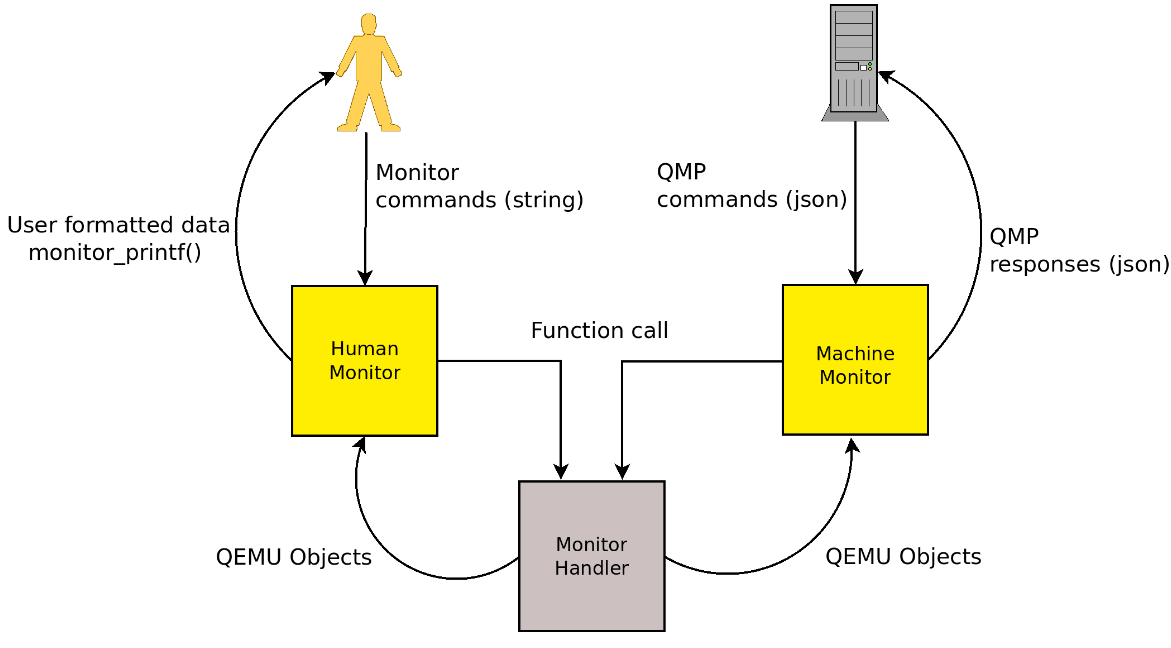
\includegraphics[]{images/qmp.png}
    \end{adjustbox}
    \caption{Схема работы QMP.}\label{fig:qmp}
\end{figure}

Libvirt -- популярное программной решение в Enterprise-разработке. Например openstack \cite{openstack}, являющийся
самым популярным облачным программным обеспечением по количеству разворачиваний, использует libvirt.
Помимо больших компаний, активно разрабатывается и поддерживается ПО, ориентированное на обычного пользователя:
Virtual Machine Manger (или virt-manager) является альтернативой таким популярным решениям как VirtualBox \cite{virtualbox} или
VMware \cite{vmware}, благодаря GUI-интерфейсу он позволяет не вводить длинные строки аргументов или писать
конфигурационные файлы.

\subsection{Объектная модель виртуального устройства QEMU}\label{sec:ch1/sec4/sub,/sub3}

Эмулятор QEMU написан в объектно-ориентированной парадигме на языке программирования C \cite{ooc}.
Хотя язык C не создавался как объектно-ориентированный язык, некоторые его конструкции позволяют
до определенной степени имитировать объектно-ориентированные подходы.
Первый компилятор языка C++ компилировал написанные программы не в машинный код, а в C, используя
его как промежуточный язык.
QEMU реализует свои механизмы и правила создания, регистрации и управления объектами, их инициализацией,
наследованием и т.п. используя в том числе библиотеку GLib \cite{glib}, в которой помимо реализации
мехнизмов ООП для языка C имеются и привычные для разработчиков высокоуровневых языков безопасные типы данных.

В QOM или Qemu Object Model \cite{qom-talking}, как и в языках, разрабатывавшихся как исконно объектно-ориентированные,
каждый созданный QOM-тип должен должен быть потомком некоторого другого типа, зарегистрированного в модели.
В терминах языка C, QOM-тип описывается двумя структурами:
\begin{itemize}
    \item структурой класса;
    \item структурой объекта (т.е инстанцированного класса);
\end{itemize}

%И массивом типа \texttt{TypeInfo}, который хранит мета-информацию о типе созданного класса.
%На \cref{fig:qom-structure} показаны отношения между составляющими объектной модели QEMU.
%Специально написанные макросы позволяют производить действия, присущие объектно-ориентированным
%языкам, вроде приведения типа объекта к типу родителя.

Базовым классом для всех классов QEMU является класс \texttt{Object}.
Наследование происходит через определение первым членом C-структуры
указателя на структуру-родитель данной. Так как язык C гарантирует, что
первый член структуры всегда начинается с нулевого отступа от начала
структуры, любой класс можно привести к типу Object.
В свою очередь Object содержит структуру, описывающую класс приведенного
объекта -- \texttt{ObjectClass}, что позволяет определить реальный тип указателя
во время исполнения.

Структуры \texttt{TypeImpl} и \texttt{TypeInfo} (см \cref{fig:qom-structure}) практически не отличаются,
но служат для разных целей:
\texttt{TypeImpl} является <<внутренним>> содержанием класса, служебной структурой,
которая скрывает методы класса от пользователя интерфейса, тогда как \texttt{TypeInfo}
наоборот, предоставляет уже очищенный от служебных полей интерфейс для инициализации \texttt{TypeImpl}.

После объявления \texttt{TypeInfo}, структура регистрируется в объектной системе QEMU.
Это происходит через использование макроса \texttt{type\_init}, который создает, можно считать,
анонимную функцию, в свою очередь вызывающую функцию \texttt{register\_module\_init}.
Созданная анонимная функция помечается атрибутом \texttt{constructor} \cite{gcc-attributes}, что заставляет
компилятор добавить вызов такой функции до вызова функции main.
Соответственно, инициализация модулей происходит до того, как начнет исполняться логика QEMU.

На \cref{fig:qom-structure} показаны отношения между составляющими объектной модели QEMU.

\begin{figure}[!htbp]
    \centering
    \begin{adjustbox}{max totalsize={\textwidth}{\textheight}}
        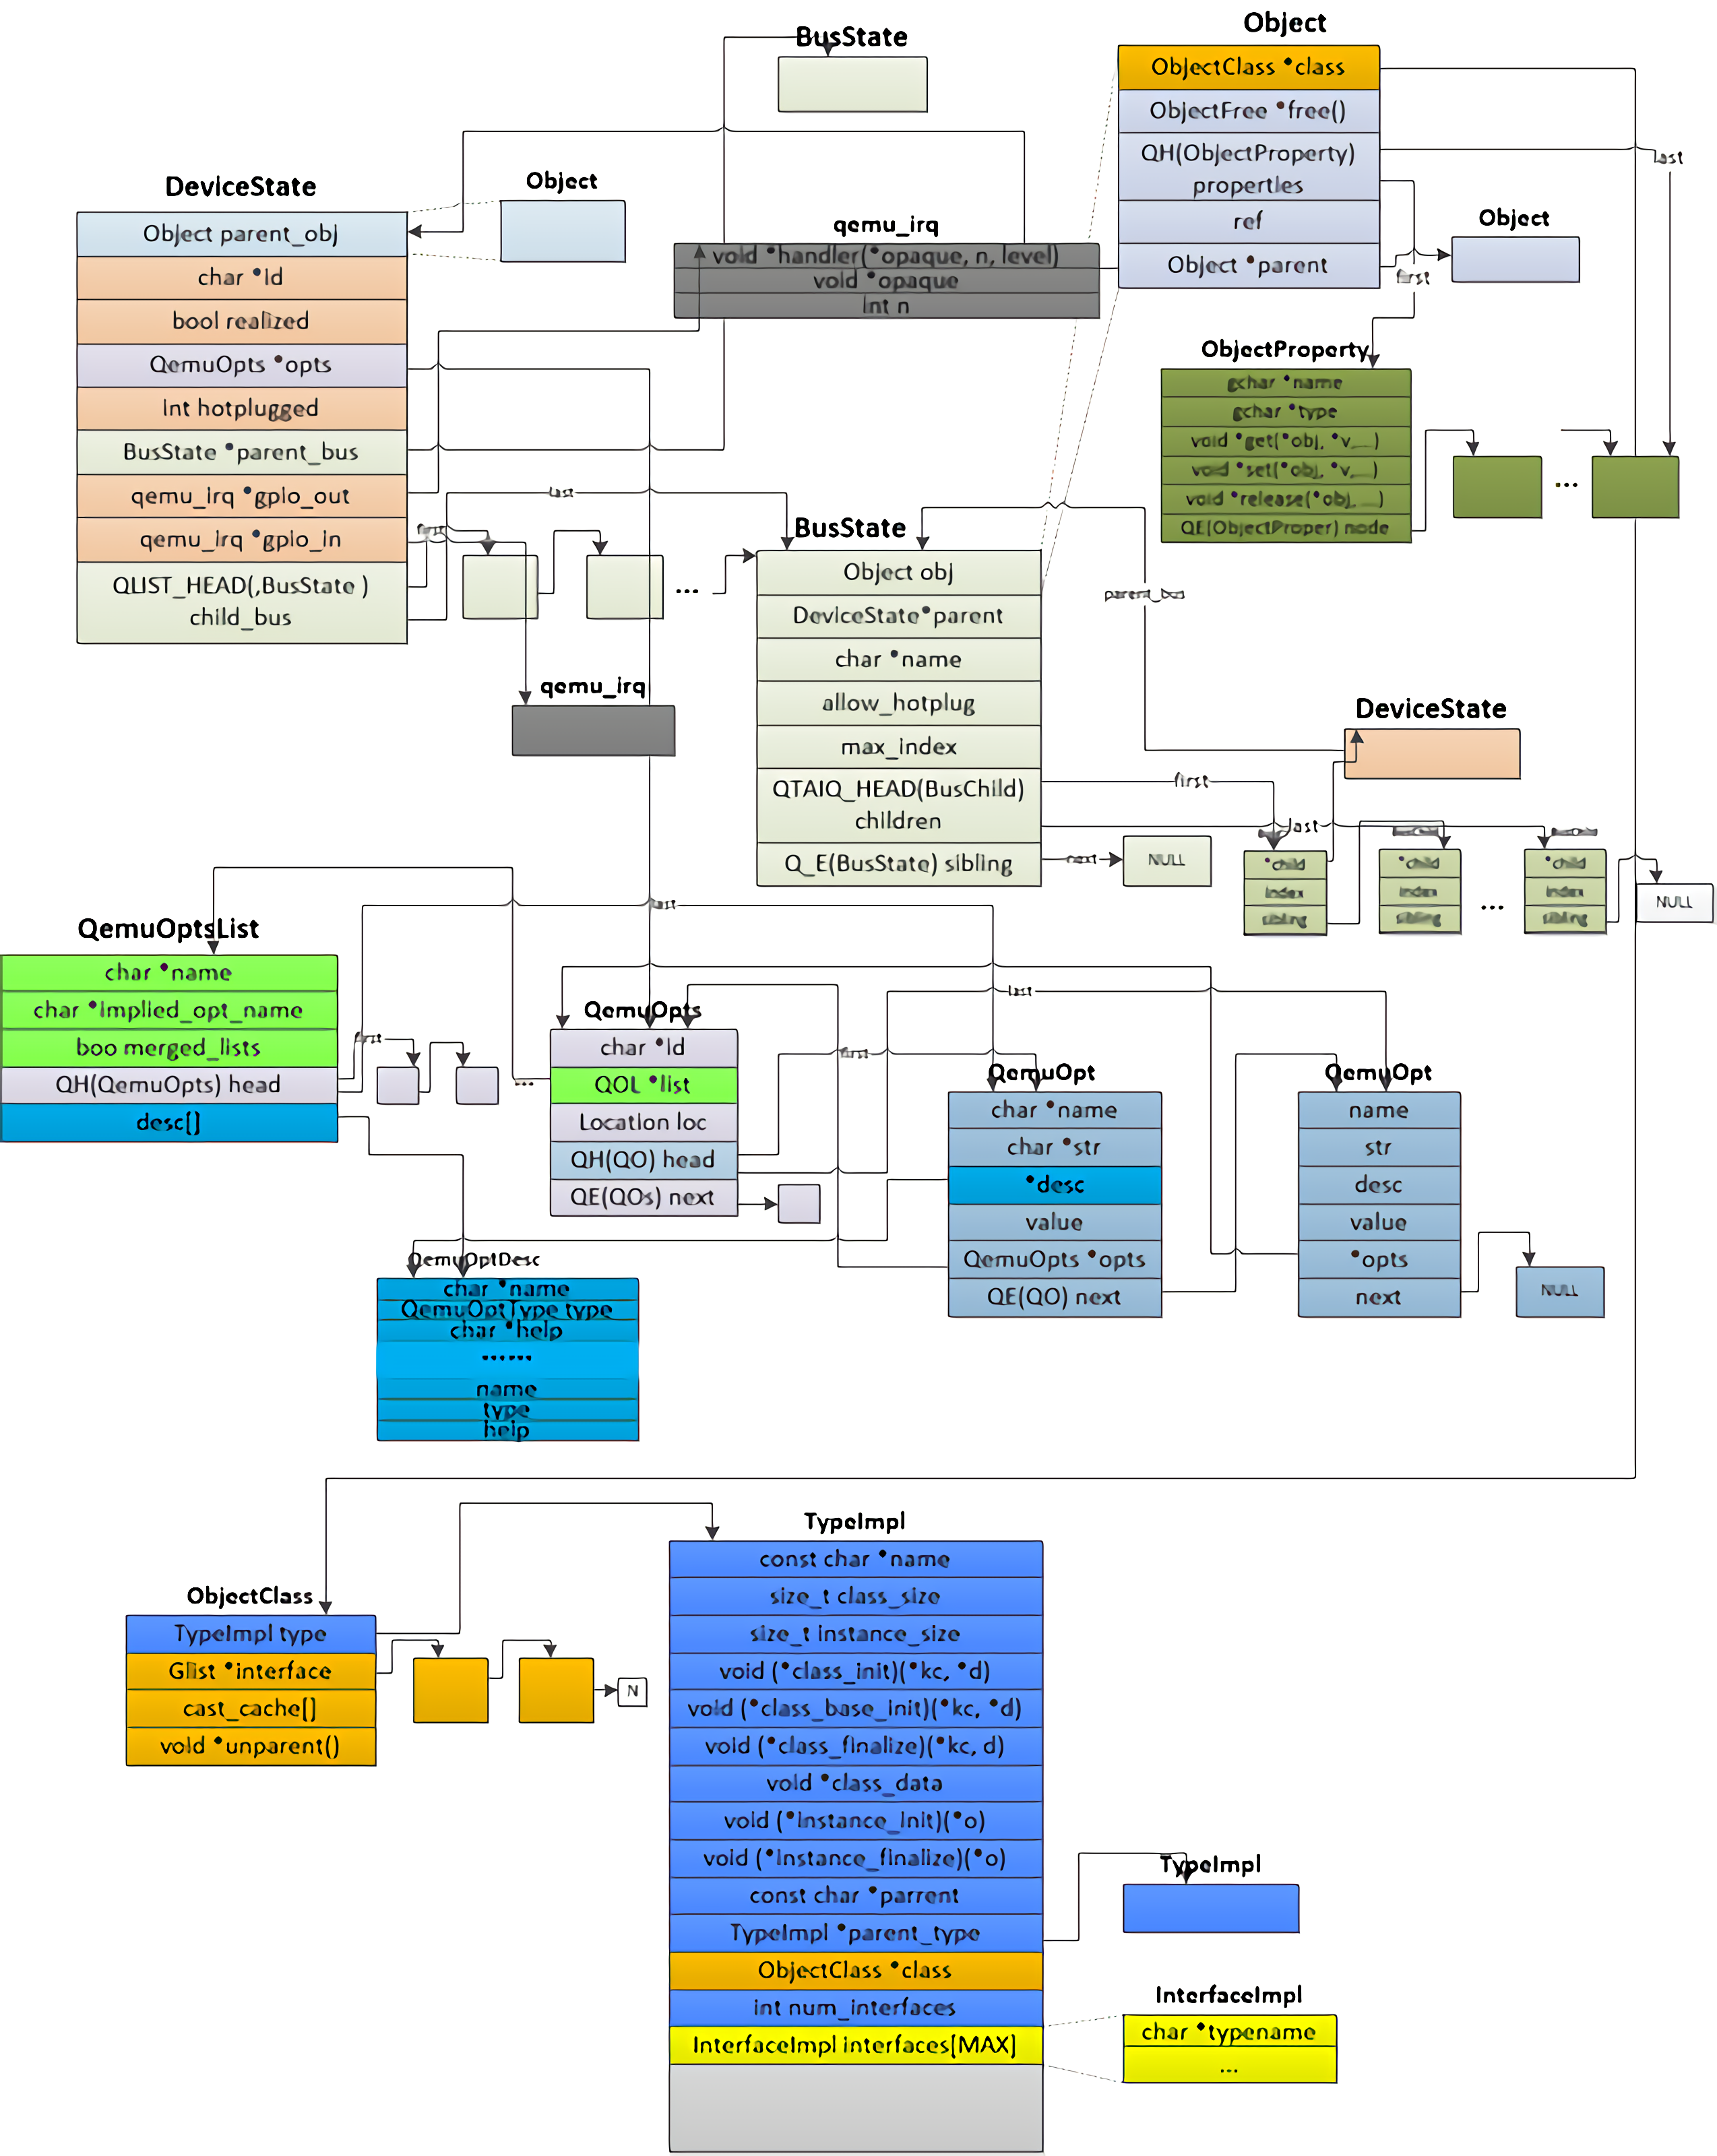
\includegraphics[]{images/qom-hierarchy_upscaled.png}
    \end{adjustbox}
    \caption{Структура QOM}\label{fig:qom-structure}
\end{figure}


% TODO: А точно ли?

Все перефирийные устройства, добавляемые в QEMU, <<общаются>> с другими устройствами через чтение и запись
по определенным для устройства адресам памяти.
За это отвечает структура \texttt{MemoryRegionOps}\cref{fig:mem-reg-ops},
которая инициализируется функциями чтения и записи,
которые вызываются, соответственно, при чтении или записи памяти, на которое <<отображено>> устройство.
Данные функции принимают на вход указатель на устройство, в чью память происходит чтение или запись,
адрес, по которому происходит чтение или запись, и, в случае чтения, количество читаемых байт,
а в случае записи -- записываемое значение и количество записываемых байт.
Некоторые устройства используют расширенные версии чтения и записи, где последним аргументом передается
структура с атрибутами транзакции.

\begin{figure}[!htbp]
    \centering
    \begin{adjustbox}{max totalsize={\textwidth}{\textheight}}
        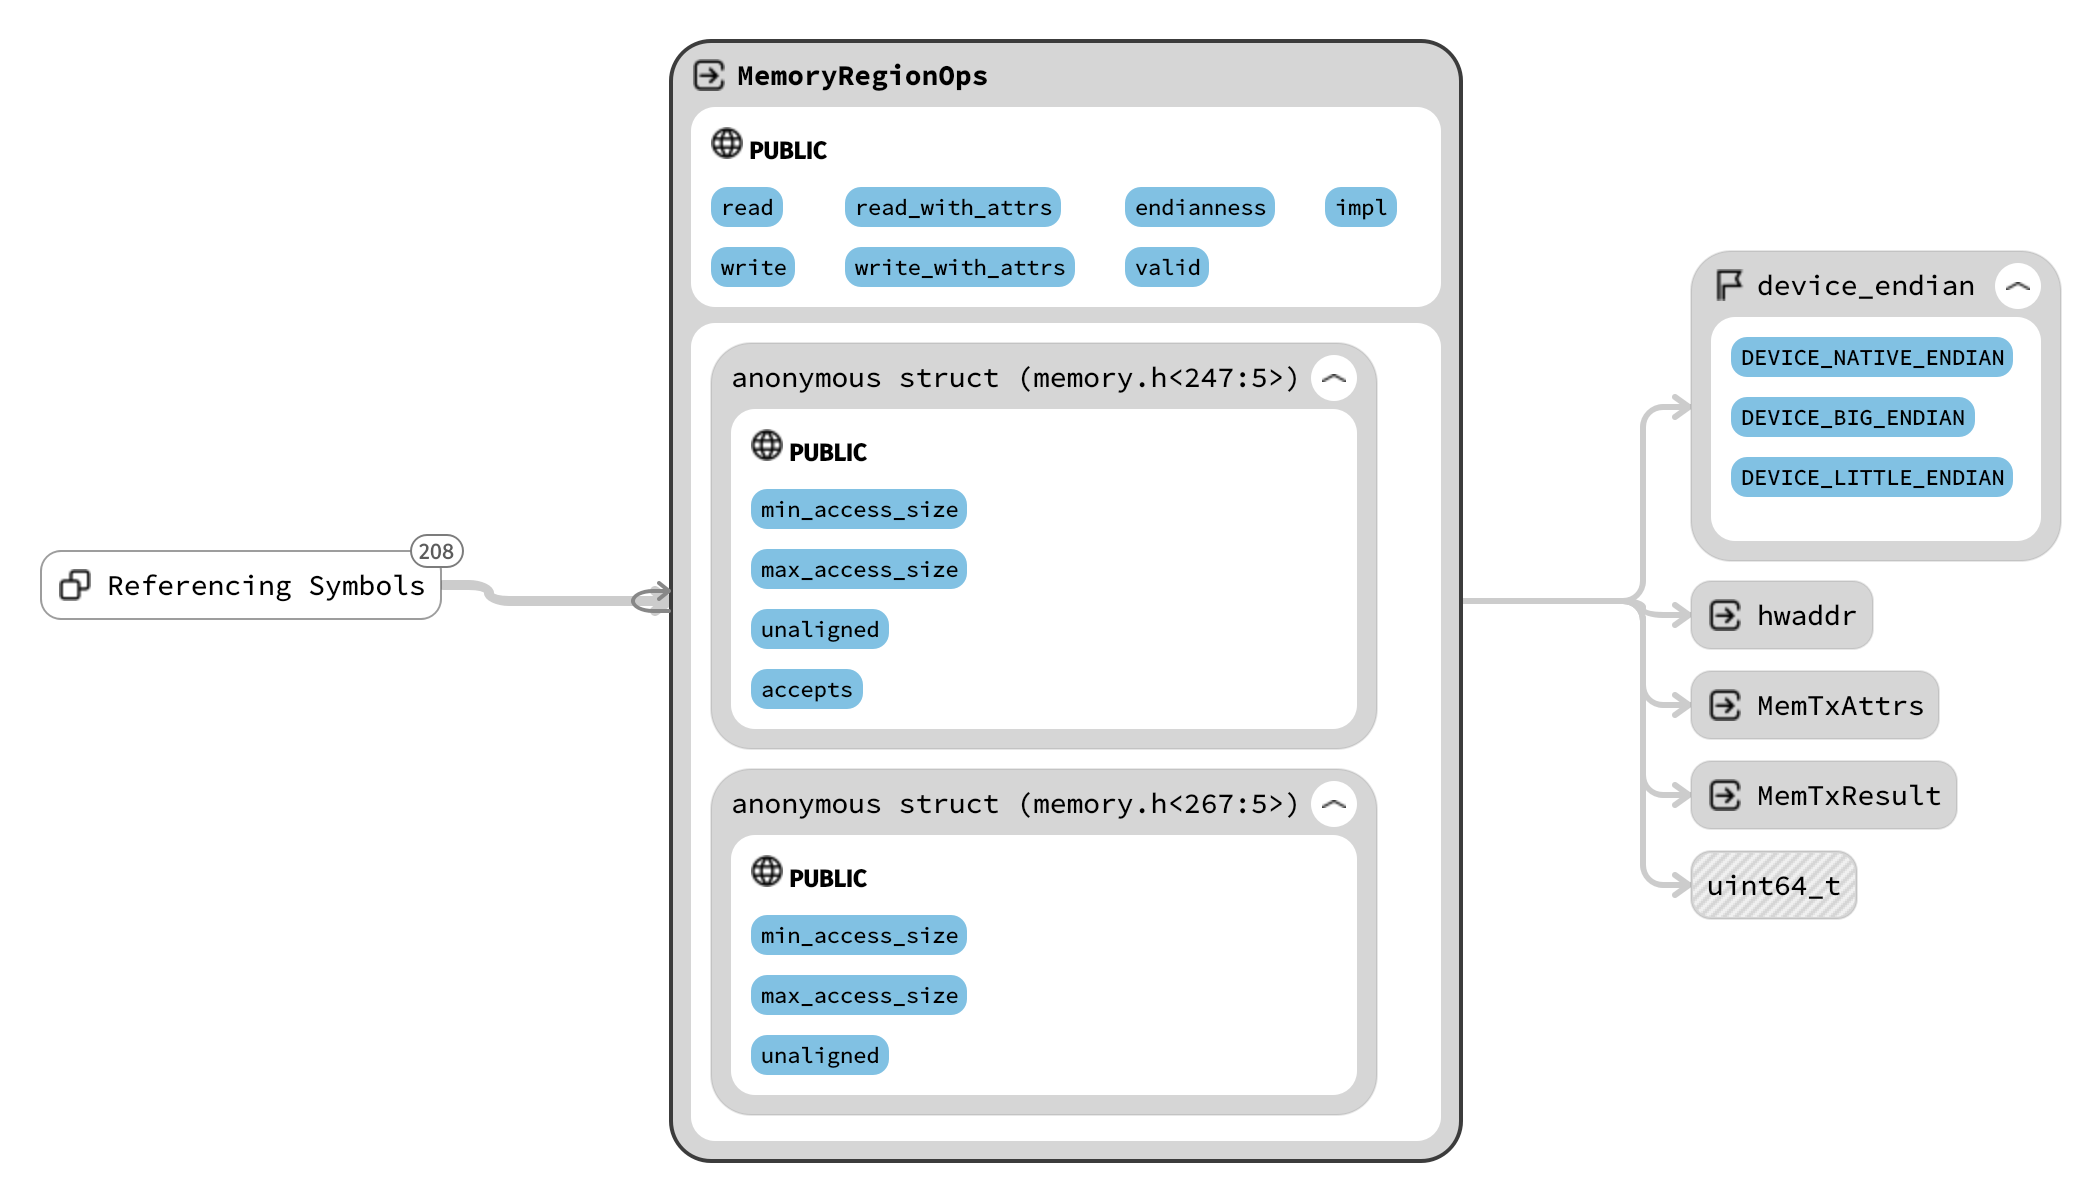
\includegraphics[]{images/mem_reg_ops_cropped.png}
    \end{adjustbox}
    \caption{Связь \texttt{MemoryRegionOps} с другими сущностями QEMU.}\label{fig:mem-reg-ops}
\end{figure}


\subsection{Встраивание нового устройства в QEMU}\label{sec:ch1/sec4/sub2/sub4}

QEMU использует QOM для описания устройств. Каждое виртуальное устройство <<подключено>> к определенной
шине. Устройства и шины формируют дерево, в котором каждый узел является либо устройством, либо
шиной. Корнем является `sysbus` <<или системная шина>>

Для встраивания нового устройства, потребуется определить структуру класса, объекта и массив с описанием
типа. Данная работа является рутинной и может быть автоматизирована с помощью кодогенератора.

Написание логики инициализации устройства может быть лишь отчасти автоматизировано, тогда как
логики работы автоматизировать не получится, но можно создать дополнительный, скриптовый,
интерфейс к C-коду, на котором описание логики устройства будет достаточно быстрым как
в смысле работы, так и в смысле временных затрат на кодирование.


\subsection{QEMU API}\label{sec:ch1/sec4/sub3/sub5}

QEMU API или сокращенно QAPI -- это программный интерфейс QEMU, предоставляющий функциональность по
управлению QEMU как для <<внутренних>>, так и для <<внешних>> пользователей.

Пользователи и процессы неявно используют QAPI, пользуясь QMP\cref{sec:ch1/sec4/sub2/sub2} или средствами
общения с гостевой системой -- QEMU Guest Agent (QGA).

QGA -- это отдельный сервис, устанавливающийся в гостевой системе и использующийся для обмена информацией
между гостевой и целевой системами, а также для выполнения команд непосредственно в гостевой системе.

QAPI имеет в своем составе генератор кода и документации из JSON-описания команд QMP.
Генератор создает все необходимые типы и функции, для получения и десериализации JSON-команд в соответствующие
C-типы, вызовы функций, запаковку возвращаемой информации пользователю.

\subsection{Сборка QEMU}\label{sec:ch1/sec4/sub2/sub6}

QEMU это большое ПО, которое написано на компилируемом языке, отчего требует
своей сборки -- нахождения используемых файлов и встраиваемых модулей,
их компиляция и последующая линковка. Разные версии QEMU построены на разных
системах сборки.

\paragraph{Makefile'ы} \cite{make} (мейкфайлы) -- это файлы определенного формата,
в которых описаны команды для сборки ПО.
Являются де-факто стандартной системой сборки в UNIX-like системах.
На мейкфайлах построены такие расширяемые проекты как Buildroot \cite{buildroot} --
система сборки встраиваемых операционных систем на базе Linux.
Сборочные системы, использующие мейкфайлы являются переносимыми, но, например в Windows
имеется собственная система сборки nmake, с несколько отличающимся синтаксисом.
Поэтому для сборки ПО классическим мейкфайлом используется либо набор программ GNUWin32 \cite{gnuwin32}, либо Cygwin \cite{cygwin} --
коллекция программ и разделяемых библиотек (cygwin1.dll) для использования POSIX API в Windows.
Зачастую используются как одна из частей Autotools \cite{autotools},
достаточно старой, неудобной и медленной системы сборки программ для UNIX-систем.

\paragraph{Meson} \cite{meson} это современная система сборки, написанная на языке Python с файлами-описаниями
сборки, похожими на синтаксис Python. Достоинствами являются:
\begin{itemize}
    \item умное пакетирование собираемых программ;
    \item кросс-платформенность системы сборки и кросс-компиляция ПО;
    \item скорость конфигурации (\cref{fig:meson-conftime}).
\end{itemize}

Meson часто используется вместе с ninja \cite{ninja} -- более быстрым,
но несовместимым аналогом make (\cref{fig:meson-conftime, fig:ninja-buildtime}).

Учитывая вышесказанное, переход на более новую версию QEMU, относительно
версии, используемой в проекте ИСП РАН (глава\cref{sec:ch1/sec2})
имеет преимущества не только для конечного пользователя, но и для разработчиков.

\begin{figure}[!htbp]
    \centering
    \begin{adjustbox}{max totalsize={\textwidth}{\textheight}}
        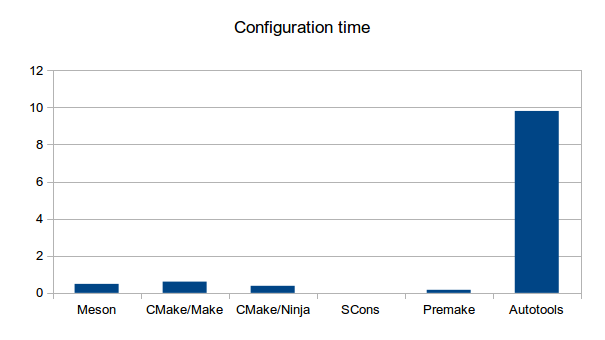
\includegraphics[]{images/conftime.png}
    \end{adjustbox}
    \caption{Сравнение скорости конфигурации meson-проекта и других систем сборки}\label{fig:meson-conftime}

    \begin{adjustbox}{max totalsize={\textwidth}{\textheight}}
        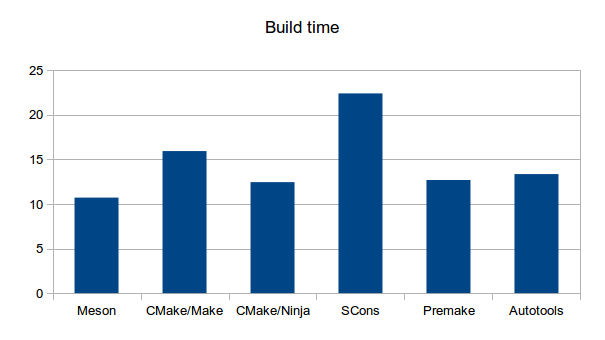
\includegraphics[]{images/buildtime.png}
    \end{adjustbox}
    \caption{Сравнение скорости сборки проектов разными системами сборки}\label{fig:ninja-buildtime}
\end{figure}


\section*{Выводы по главе}\label{sec:ch1/sec5}\addcontentsline{toc}{section}{Выводы по главе}

Представлены области применения виртуального аппаратного
обеспечения.

Осуществлен аналитический обзор существующих методов и средств
создания виртуального аппаратного обеспечения, который показал
актуальность разработки DSL-языка для описания виртуального аппаратного
обеспечения, алгоритма и методики его применения.

Поанализированы существующие подходы к созданию виртуального
аппаратного обеспечения. Рассмотрены преимущества и недостатки
разработки ИСП РАН.

Сформулированы цели и задачи диссертационной работы, состоящие в
снижении времени разработки и трудоемости создания виртуального
аппаратного обеспечения.

Рассмотрен эмулятор QEMU:
\begin{enumerate}[label={\arabic*)}]
    \item Архитектура QEMU;
    \item QEMU Machine Protocol;
    \item Объектная модель QEMU (QOM);
    \item Процесс встраивания виртуального устройства в QEMU;
    \item Программный интерфейс QEMU (QAPI);
    \item Процесс сборки эмулятора;
\end{enumerate}
